%section: Ransomwares and ransomware attacks
%last subsection: how to get infected
    \subsection{Encryption mechanism: how do ransomware work}
        Once the malware starts running on target computer, it generates a random symmetric key\footnote{used both to encrypt and decrypt information}, usually one per file, and it encrypts each file with it.\\
        The symmetric key itself it's encrypted with a public key, of an asymmetric key pair generated on the server of the group that runs the malware. The private key is stored on the server, and it will released only when the ransom is payed.\\
        Most of this process is automated: when cryptocurrencies are transferred to the criminals' address, the server releases the key associated to it.
        Different keys to allow the attackers to decrypt only a part of the samples to demonstrate that they can do it.
\section{Indirect monetization: Botnets}
    The word botnet comes from the words \textit{robot} and \textit{network}. A botnet is composed by few hundreds to millions of infected devices which run some sort of malware they got by opening an infected email attachment, by plugging an infected USB drive, visiting an infected website \textit{(these are examples of ways to get infected)}\\
    Each botnet has a \textbf{botmaster} who controls and rents it out to perform tasks \textit{(denial of service, spamming, phishing campaigns, crypto mining \dots)}, and his only objective is to earn money by renting them.\\
    The significant challenge with this type of crime is that each bot per-se is not dangerous for the machine itself, but for other machines, and since the cost of cleaning up a machine falls on its owner, some can decide to not do anything about. This cost can be seen as a small fee to be payed by \textit{the community} to get everybody safe. Like a vaccination, some cases of infected machines are not a big trouble for the community, while a lot of them can be really dangerous for everybody.
    \subsection{Rise of the bots}
        Back in the days botnets were used to control IRC chats \textit{(see IRC wars)}. Then instead of using the compromised machines to control the chat, botmasters started to use the chat to control the bots.\\
        In 1999, there was one of the first DDoS attacks, which was against University of Minnesota and used at least 227 bots.\\
        In the 2000s DDoS attacks against high profile websites \textit{(Amazon, CNN, eBay \dots)} got huge media coverage.
\newpage
    \subsection{Geolocalization of botnets command and control}
        \begin{figure}[ht!]
            \centering
            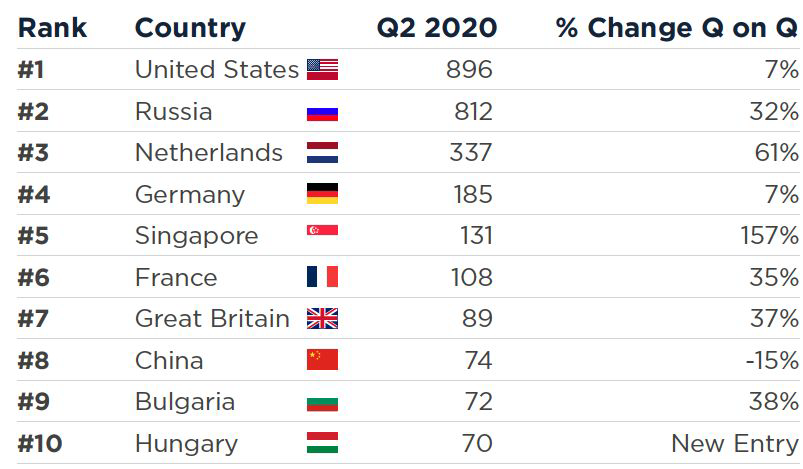
\includegraphics[width=0.6\linewidth]{chart.png}
        \end{figure}
        This chart shows the number of new botnet C\&Cs detected by \textit{Spamhaus} in the second quarter of 2020, and the increase wrt the first one.\\
        By keeping in mind the \textit{observation bias}, we can also introduce another kind of bias which is called \textbf{heatmap effect}: we're biased on the density of the population and on how much data we collect from a certain country.\\
        In this kind of charts we'll always have U.S.A. on top, because there's more penetration in the internet, and also this kind of things is tracked. While we'll have less data from less technological advanced states or \textit{perfectly democratic countries} like Russia or the P.R.C. which can result in lower positions while in reality being the first ones.\\
        Here we see an important increase of C\&C from The Netherlands:
        \begin{itemize}
            \item it is possible that \textbf{something is on}
            \item or simply that some Netherlands organization decided to participate in this data collection feeding a lot of \textit{new} data
        \end{itemize}
        Funny thing about Russia and P.R.C: Russian people hack russian computers too, while P.R.C citizens don't hack into their fellows machines.
\newpage
    \subsection{Type of (botnet) malware families}
        \begin{figure}[ht!]
            \centering
            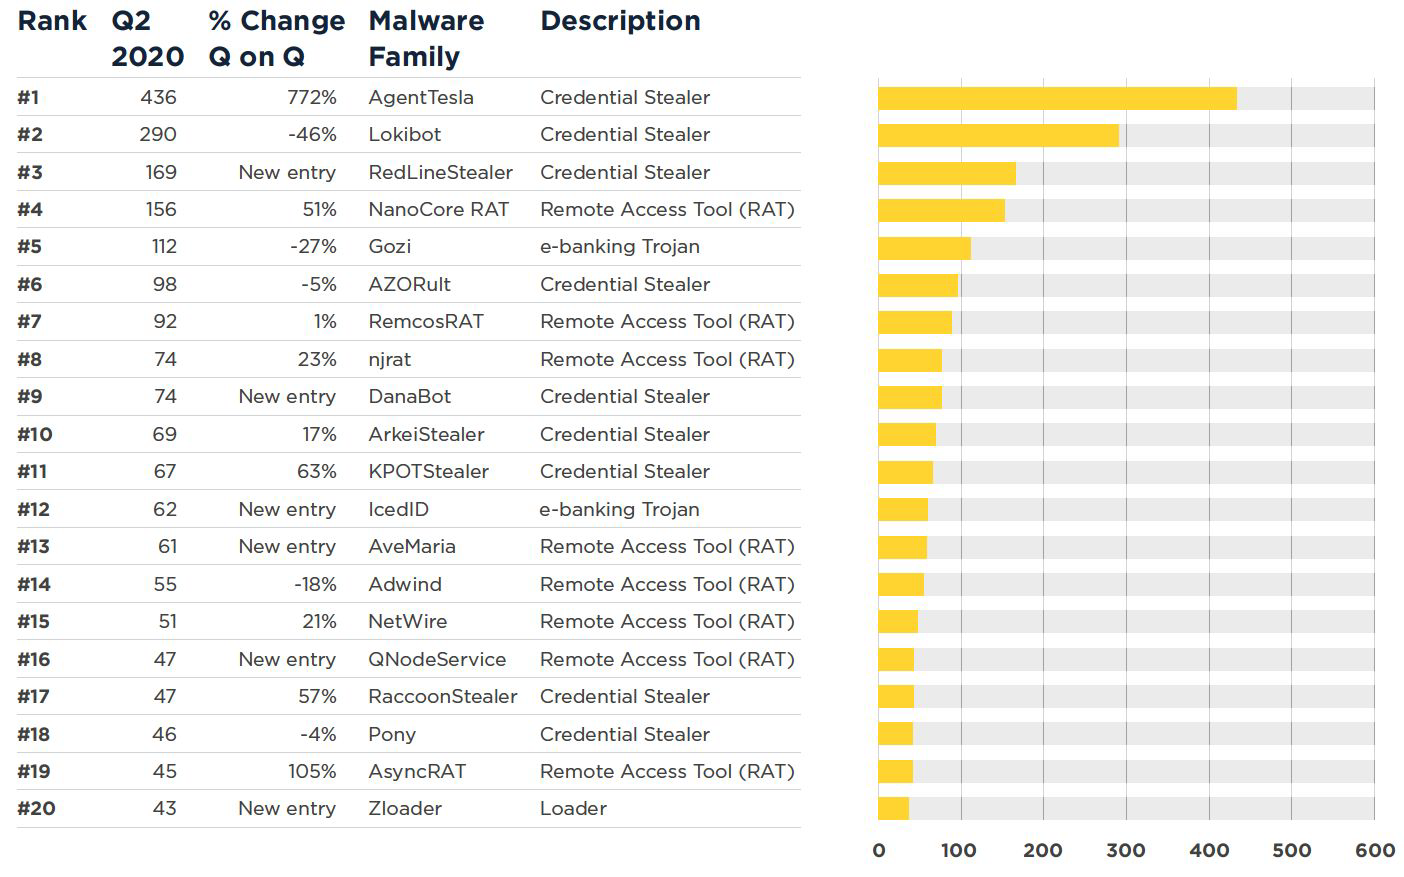
\includegraphics[width=0.6\linewidth]{families.png}
        \end{figure}
        Every botnet in general can be used to do any sort of things, but they're used to do only one of them:
        \begin{itemize}
            \item \textbf{Credential Stealers:} used to steal sensitive credentials.
            \item \textbf{Banking Trojans:} credential stealers specifically designed to perform stealing of bank accounts information. \textit{(Gozi is the most common one, Zeus the most important one)}
            \item \textbf{Remote Access Tools:} basic botnet oriented malware, which allows to control a computer in order to perform whatever.
            \item \textbf{Loaders:} specifically designed to allow a botmaster to load a program of whatever sort on a computer. Maybe a client ask you to install a certain malware on a lot of computers, and you can do it with a loader.
        \end{itemize}
        We talk about families because there are criminal groups that only develop their source code, and who performs the attacks buys the code and personalizes it for the specific purpose they need.\\
        So we can consider three businesses: how to develop them, how to configure them, how to use them.\\
        There is a market for services related to malwares and cyber attacks \textit{(cybercrime as a service, underground market...)} structured around the needs of cyber criminals. This market is fueled by the money that these schemes make. Some of these money pays for the tools used to make that money.
\newpage
\section{The cybercrime ecosystem}
    The status quo consists in \textbf{organized groups} performing \textbf{various activities:}
    \begin{itemize}
        \item Development and procurement of exploits
        \item Site infection
        \item Victim monitoring
        \item Selling \textit{exploit kits}
    \end{itemize}
    \begin{figure}[ht!]
        \centering
        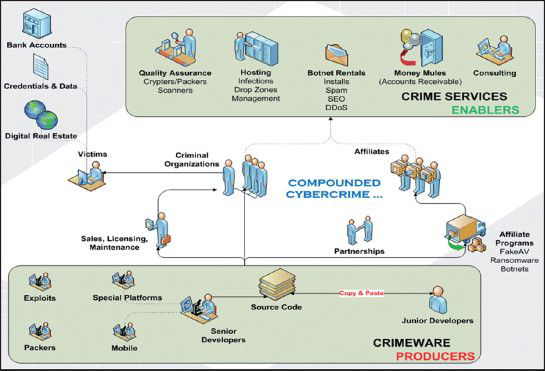
\includegraphics[width=0.6\linewidth]{ecosystem.png}
    \end{figure}
    These ecosystems can exists because some of the activites done are not illegal: developing exploits per-se is not illegal, selling one is not illegal, the usage of them may be or may be not illegal.
    Even the services related to the configuration of malware are not illegal, while execution and operation may be.
    If you're sufficiently shielded and you run these \textit{businesses} in countries that cannot persecute you, we can even know your name and surname but you cannot be arrested.
    \begin{itemize}
        \item Developers write the source code for malwares with the help of packers and exploits developers
        \item Crime service enablers:
        \begin{itemize}
            \item Quality assurance makes sure that antiviruses don't detect their software
            \item Bulletproof hosting is a kind of \textit{close-an-eye} hosting, \textit{(e.g. russina business networks)} with permit certain suspect activities over their infrastructure, they're sort of borderline organization with lot of regular customers, and some bad ones
        \end{itemize}
    \end{itemize}
    \subsection{Identity sales}
        People's identities are sold on the black market. They are worth because they can be used for fraud, to open bank accounts used for money laudering for example.
        The more they're useful, the more they are worth.
        Worth 50 dollars for you that sell it, the one who pays is going to use them for fraud which is worth more.
        The black market is fueled from an enormous amount of money that people stole.
    \subsection{Drive by download}
        \begin{figure}[ht!]
            \centering
            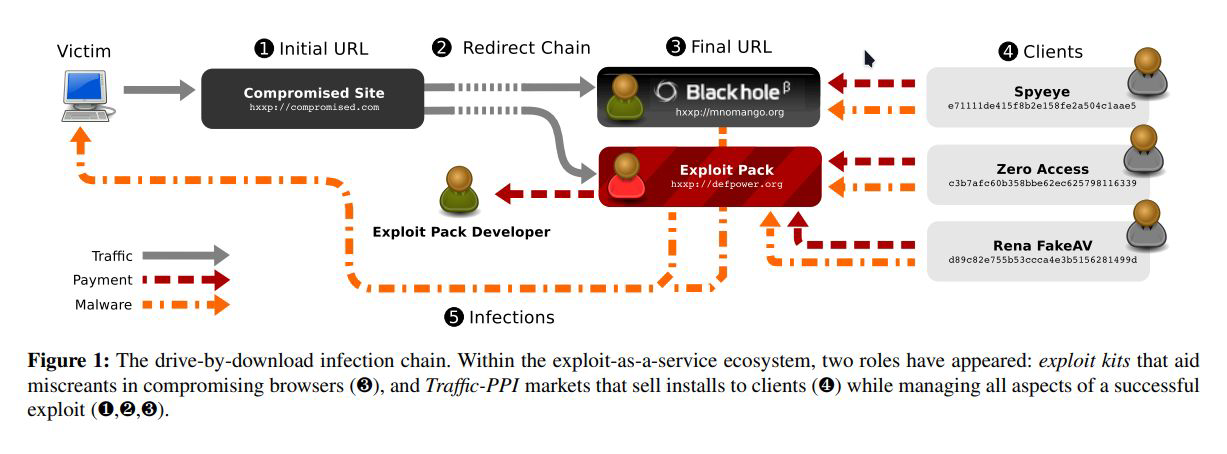
\includegraphics[width=0.6\linewidth]{drivebydownload.png}
        \end{figure}
        This is another way in which malwares are installed:\\
        an exploit breaks into your browser and executes code on your machine. This requires your browser to be vulnerable and for you to visit a compromised website with the exploit running \textit{(streaming, cracks of programs websites,\dots)}.
        The most compromised are \textit{factually illegal websites}: you're not scared of the strange url if you are in need to see the last movie in streaming, download the expensive program's crack, this is in contrast with a normal situation like going to amazon to buy shoes.\\
        But, \textit{traps} can be also present in legitimate websites.\\
        What actually happens is that the users endup in a series of redirects, called \textbf{redirect chain}, which will endup in a visit to a website running what is called \textbf{exploitation pack} for your browser.
    \subsection{Exploitation kits sales}
        This kind of kits is sold in the dark web by well known organizations, take \textit{Blackhole} as example:\\
        they were buying exploits from developers to earn 10s of millions per month renting them.\\
        Their boss, surprisingly called Dmitry “Paunch” Fedotov, was arrested in 2013 after years of running the website.
    \subsection{Monetization on the dark web}
        Monetization takes a lot of forms, one of them is stealing credit card numbers to sell them for a relatively small price.\\
        The hackers get \textit{easy and fast} money, while the buyers need to use the real money on the cards to buy expensive objects or to start frauds because they can be easily refunded. \textit{(apple computers, ethnic travel example..)}.
    \subsection{Cybercrime and perception}
        Online, you detach people from the picture. It's actually easier to commit crimes, it's easier to crack a program instead of stealing a car, lot of cyber criminals would never be criminals in the real world.
        But when you do cybercrime, your perspective is different: you have another perception of what you're doing, that's the reason because crime happens more online.\\
        Ethical people understand the consequences of their actions, and may decide to not do them, but someone can not care about what can happen as a consequence of their actions and perform them anyways:\\
        in the Jamal Khashoggi case, the exploiter which wrote the code for the spyware that ended up to make him killed, would never kill someone. But the consequences of his actions did.
    \subsection{Money mules and money laundering}
        Most cybercrimes end up with a digital form of money, which crimials want to bring in a physiscal form, completely disconnected from what they did in principle.
        \begin{itemize}
            \item They can pay invoices to companies somewhere in the world, which in a certain way makes sure that the money come back clean. \textit{(traditional way)}
            \item They can make use of \textbf{money mules}
        \end{itemize}
        Money mules are intermediary people which by purpose or not make earnings coming from cybercrime clean money.\\
        Accomplished ones may be people that have nothing to lose \textit{(prejudiced, poor people \dots)}, they just open bank accounts by their names and get the money transferred and then withdrawn and handed to criminals.\\
        Some of them may also open accounts by somebody else's name using identities that may be stolen with an attack and bought online. They're most difficult to catch because the Police needs to be actually there while they are withdrawing money.
        \\Unaccomplished ones may be people which are fooled by things like the Nigerian prince scam: they get the money on their bank account, send 70\% of them to criminals in packages or by moneytransfer, and keep 30\%. Most of the cases they get arrested and have to pay back all the money, also the ones they don't own no more.\\
        Buying and selling of goods \textit{(ricettazione)}, videogames curriencies, \dots, are other ways to perform money laundering.
\chapter{Cryptocurrencies: abuses and forensics}
    We talk about cryptocurrencies in the way they are used in cybercrime.
    \section{Bitcoin and blockchain}
        Bitcoin is an attempt to create \textbf{electronic cash}: a digital currency that has lots of properties that physical money have, one of them is \textbf{no central authority}.\\
        What Satoshi Nakamoto wanted to have is an electronic distributed ledger\footnote{ledger=registro}.\\
        Having no central authority is a really hard problem to solve \textit{(byzantine consensus)}, he did it with \textbf{the blockchain}.\\
        The blockchain is a \textbf{shared, append-only, trustable} ledger of all coins transactions. The limits of distributed consensus defined in the Byzantine Problem and CAP Theorem are solved using the technique of \textbf{proof-of-work}.
    \section{Wallet and addresses}
        A wallet is the software that allows to manage and store the \textbf{public} and \textbf{private} keys for each of the user's bitcoin addresses. To create and sign transactions, track the balance.\\
        A bitcoin address is an alphanumeric string which identifies a \textit{point} where you can send bitcoin to, and where they can be sent from.
        In order to know how many Bitcoin are \textit{stored} in that key you need to go to the origin of all the transactions and track the flow of them to understand how much of them are there now. This computations is not really efficient but can run without central authority, so the only reason for using a blockchain is if it is really so important to get a way out of a central authority.
    \section{The bitcoin transaction life cycle}
        \begin{figure}[ht!]
            \centering
            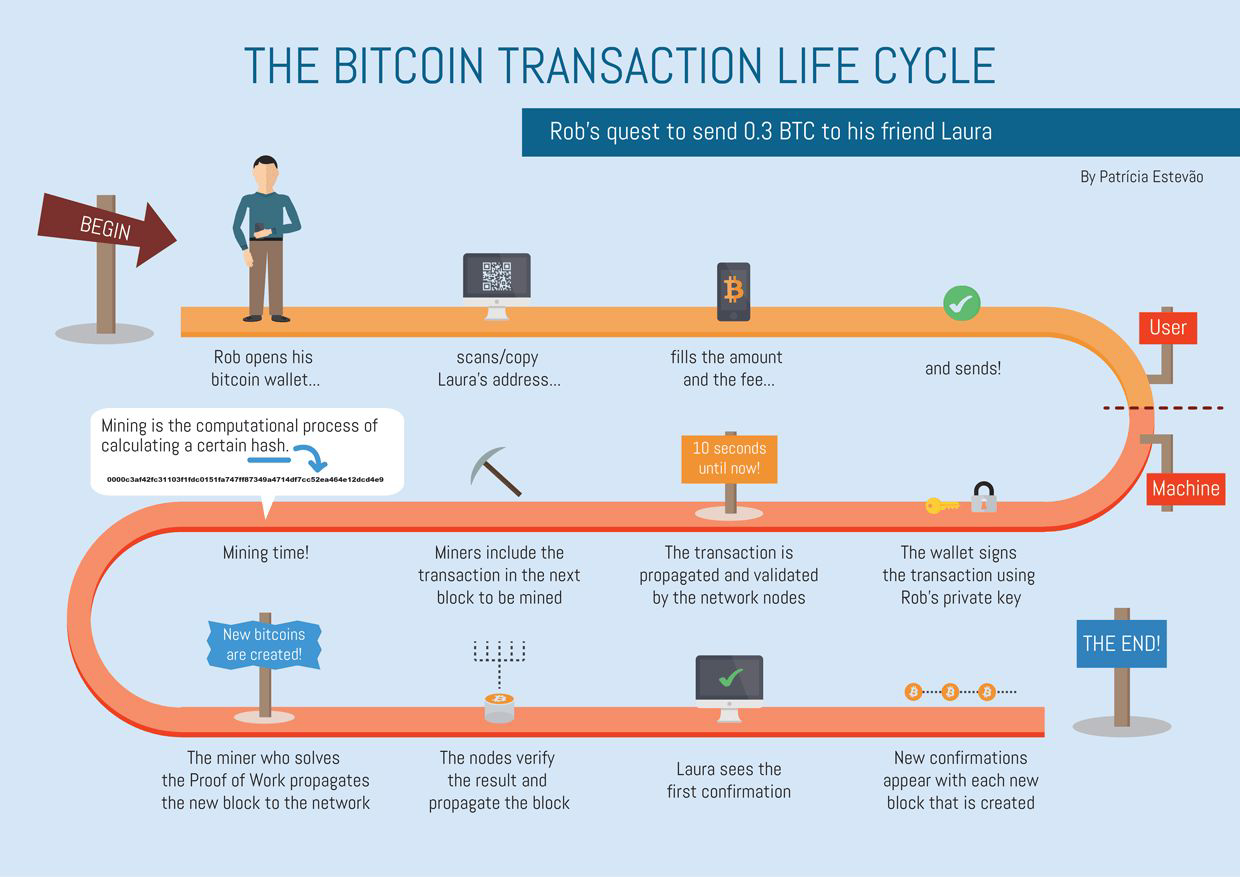
\includegraphics[width=0.6\linewidth]{lifecycle.png}
        \end{figure}
        As soon as the transaction is on the immutable ledger, the money are on the other address. How do we ensure that this is the only transaction done with those Bitcoins?\\
        Our immutable ledger must be consolidated, with a central authority that would have been easy, how do we agree with no central authority? We need a history that cannot be modified, and to do this we talk about mining.\\
        Mining is the process to generate a block containing all the transactions, and to append it to the blockchain.
    \section{Mining}
        Miners compete to generate a new valid block that solves a complex mathematical problem bybruteforce: the solver is then rewarded a fixed number of BTC.\\
        It is a computational demanding activity: miners put a set of transactions in the new block, put there a destination for the reward and then start bruteforcing the block to find a sha256 hash of it which starts \textbf{with a certain number of zeros}. The more zeros, the more difficult is the process.\\
        When a block is added to the blockchain, the other miners stop bruteforcing their blocks and start to compute the hash of another one, to link it to the last found block.
        The difficulty increases more and more, the reward got smaller and smaller but BTC value gets larger and larger.
    \section{Fork events}
        Sooner or later two miners will get a solution at more or less the same time. This causes a fork where the situation is that for some miners the blockchain ends with block A and for some others with block B.\\
        Now the blockchains are two, and sooner or later some miner will find a solution and append a new block in one of them. The rule says that \textbf{the longerst blockchain is the true one}. As soon as one blockchain becomes longer, all the miners move to that leaving the other one sadly alone.\\
        This is done because in order to revert a payment you'd need to go back on your block, go ahead mining until your blockchain is the longest one: this means that you would compete with all the other miners.     